\subsubsection{Text Analysis}

To better understand the TextVQA dataset from the language perspective, we conduct an analysis on the questions and answers on all three data splits. TextVQA contains 45336 questions in total, of which 37912 are unique. Following the original paper, we visualize the distribution of question lengths on all three data splits in Figure \ref{subfig:qlength}. Since the TextVQA validation and test split are randomly sampled, the distribution is almost identical across data splits. The average question lengths in the three data splits are 7.18/7.21/7.11 respectively. As shown in Figure \ref{subfig:top10start}, more than 78\% of the questions in TextVQA are what-questions. We also show the 10 most frequent questions and their frequency in Figure \ref{subfig:top10q}. The distribution of the 10 most frequent answers is shown in Figure \ref{subfig:top10a}. It is worth noting that more than 600 questions are labeled as unanswerable while more than 400 questions are labeled as ``answering does not require reading text in the image''. Other answers in TextVQA include various entity types like numbers, brands, cities, time, and people's names.

    
%%%%%%%%%%%%%%%%%%%%%%%%%%%%%%%%%%%%%%%%%%%%%%%%%%%%
\begin{figure*}[h]
  \centering
  \begin{subfigure}[b]{0.8\textwidth}
    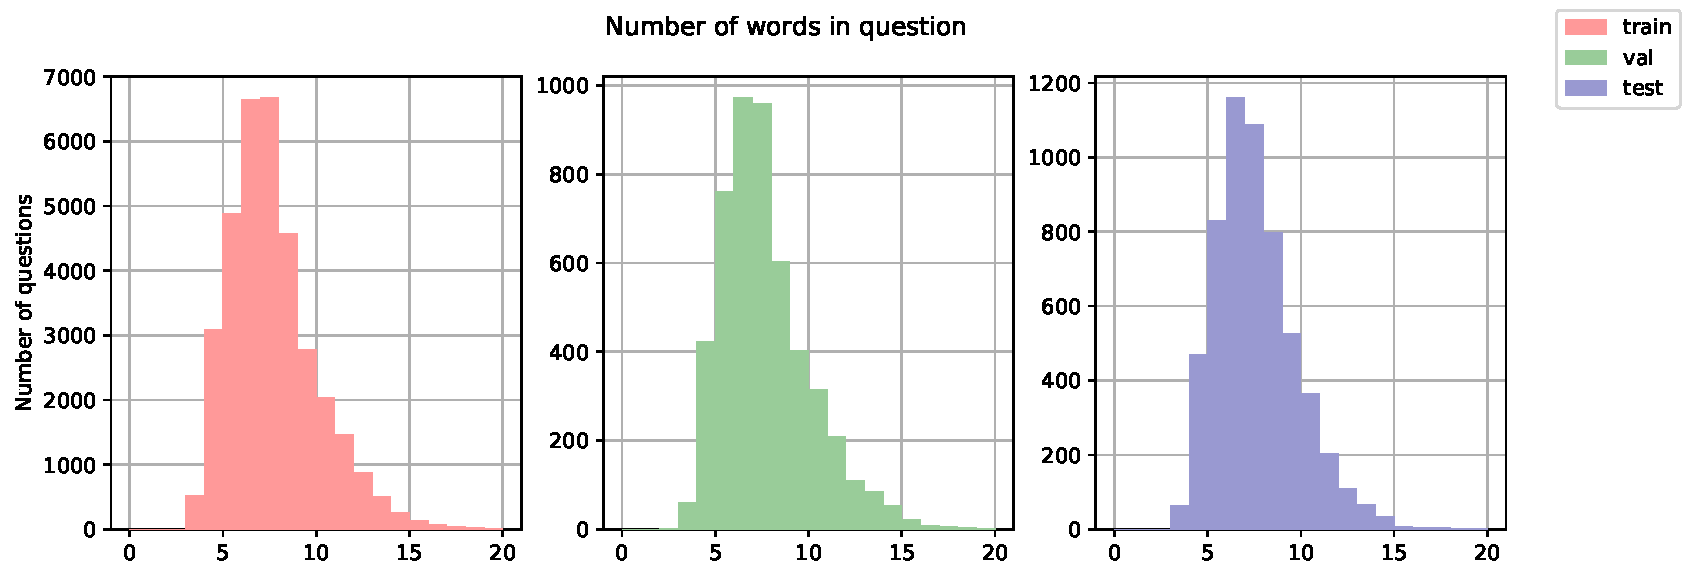
\includegraphics[width=\textwidth]{figures/qlength.pdf}
    \caption{}
    \label{subfig:qlength}
  \end{subfigure}
  
   \begin{subfigure}[b]{0.8\textwidth}
    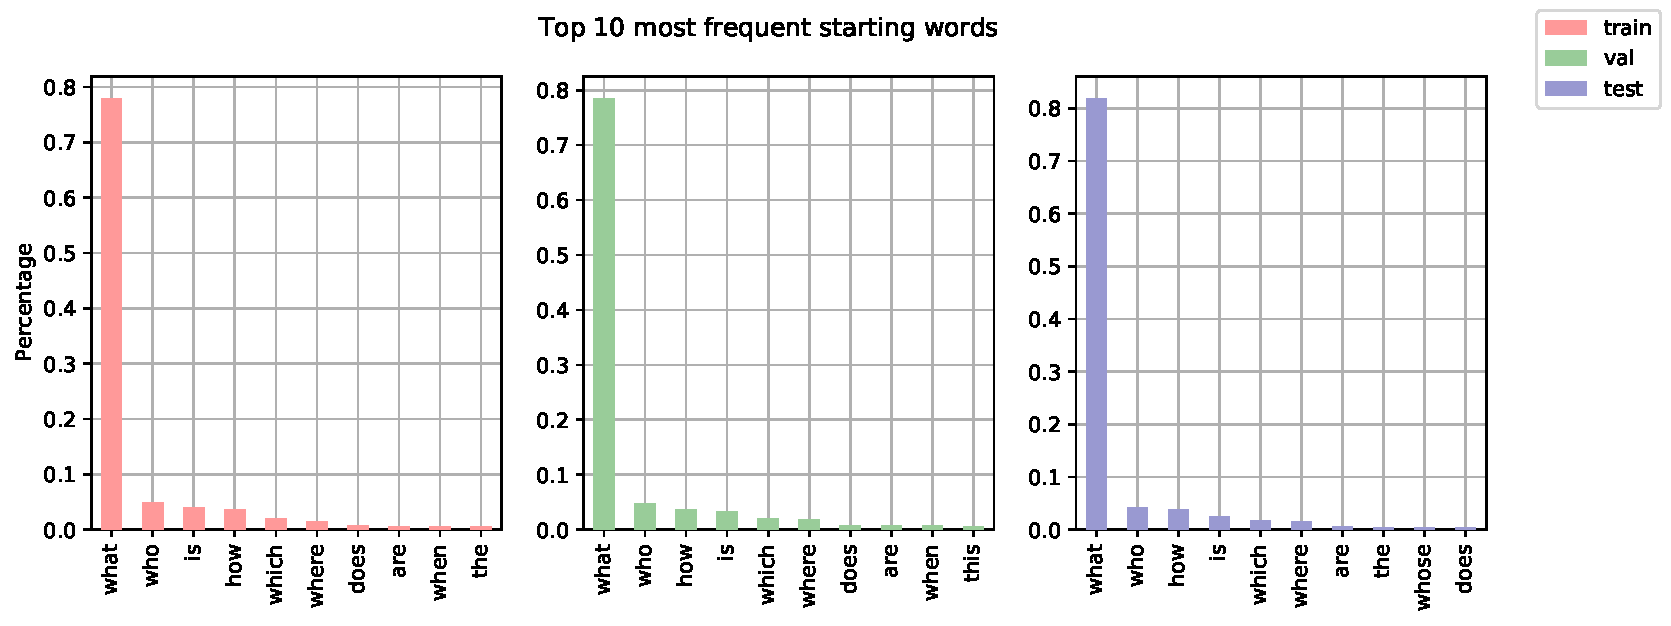
\includegraphics[width=\textwidth]{figures/top10start.pdf}
    \caption{}
    \label{subfig:top10start}
  \end{subfigure}
  
  \begin{subfigure}[b]{0.8\textwidth}
    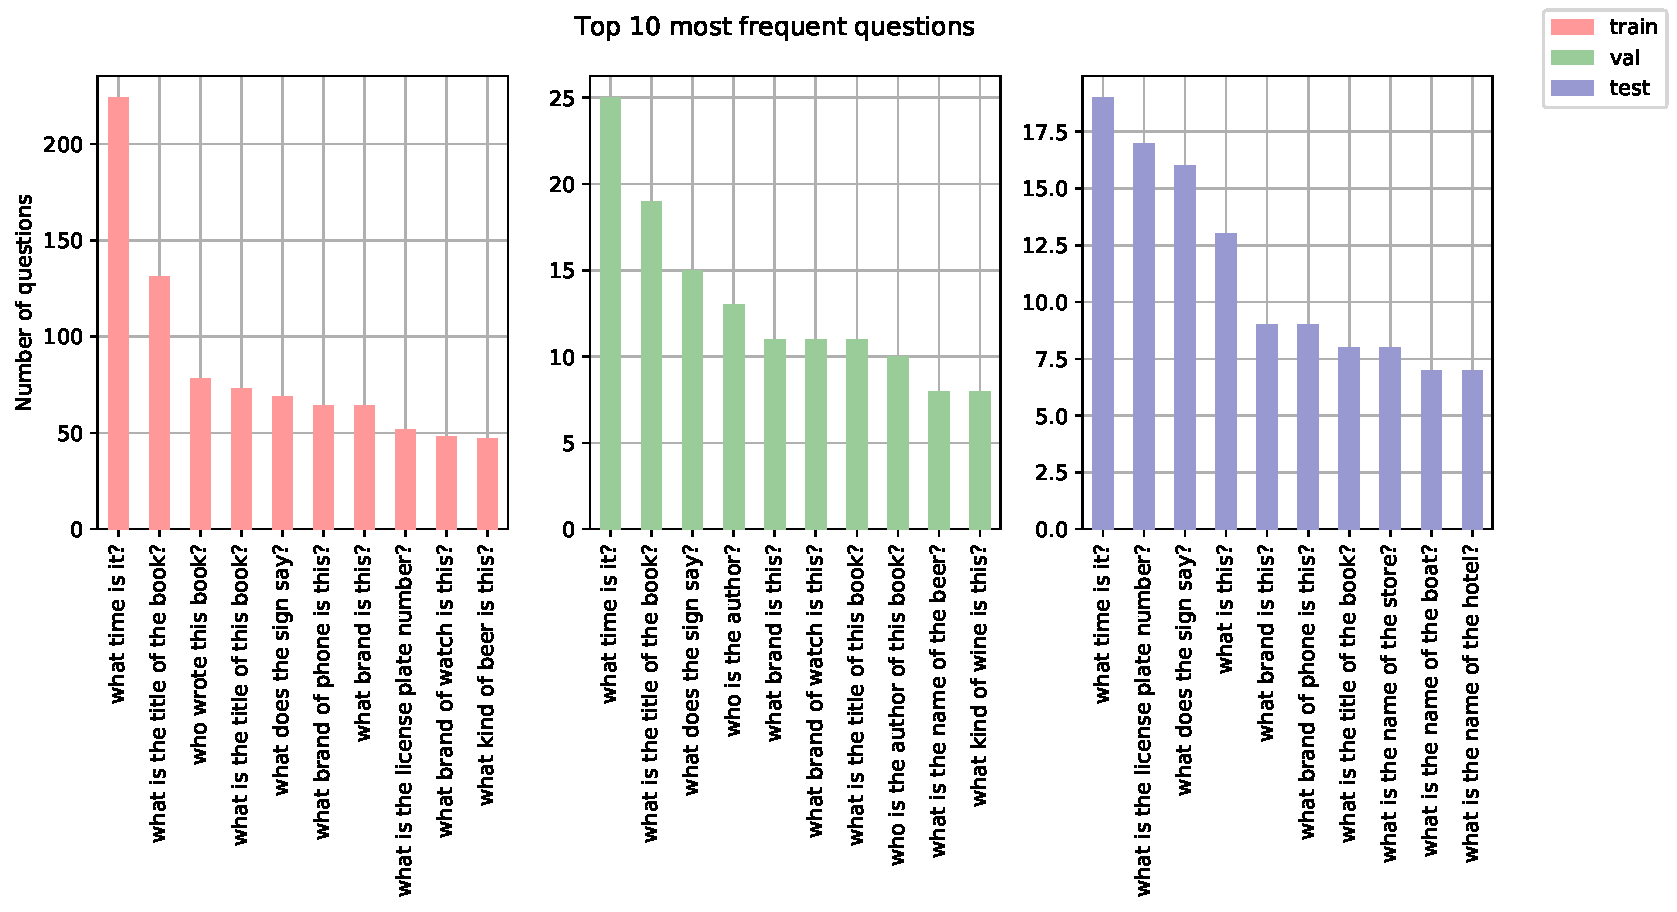
\includegraphics[width=\textwidth]{figures/top10q.pdf}
    \caption{}
    \label{subfig:top10q}
  \end{subfigure}
  
  \begin{subfigure}[b]{0.5\textwidth}
    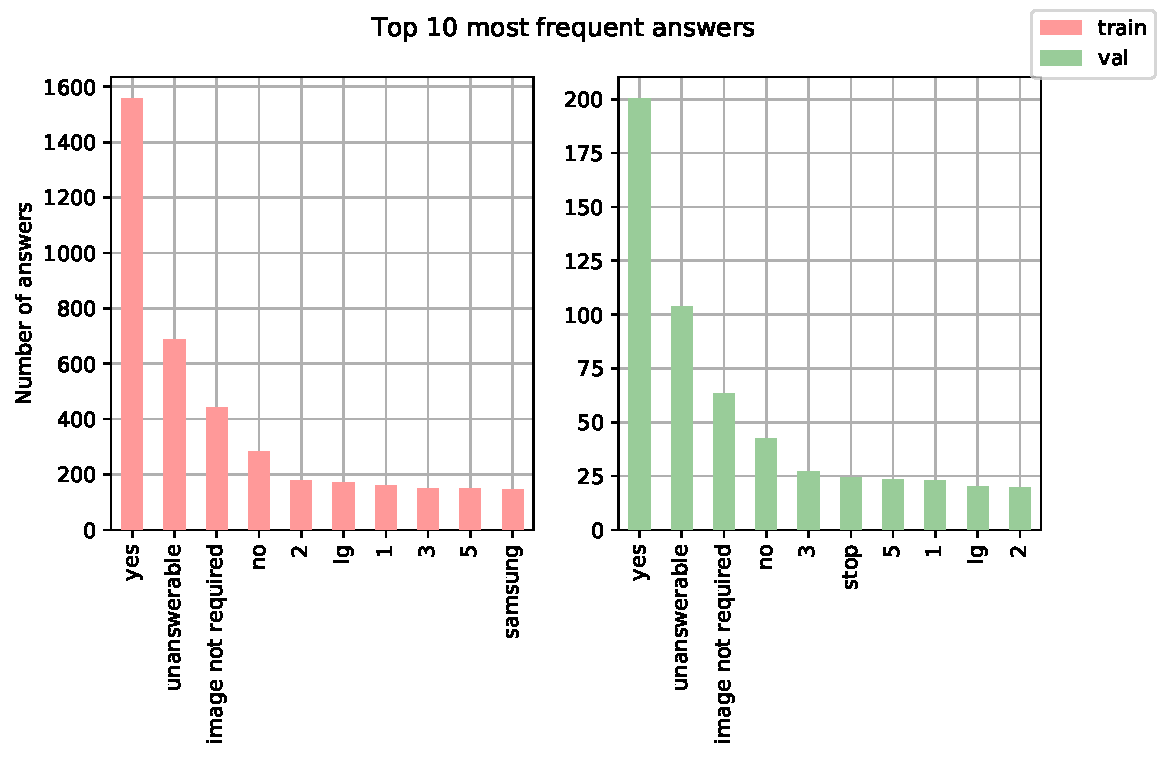
\includegraphics[width=\textwidth]{figures/top10a.pdf}
    \caption{}
    \label{subfig:top10a}
  \end{subfigure}

  \caption{Text statistics of the TextVQA dataset.}
  \label{fig:asdf}
\end{figure*}
%%%%%%%%%%%%%%%%%%%%%%%%%%%%%%%%%%%%%%%%%%%%%%%%%%%%